\documentclass[12pt]{article}
%\usepackage{fancyvbr, pstcol}
%\setlength{\parskip}{1ex plus 0.5ex minus 0.2ex}
\setlength{\parskip}{1em}
\parindent0mm
\textwidth150mm
\textheight200mm
\oddsidemargin+5mm
%\usepackage[dvips]{graphicx}
\usepackage{color}
\usepackage[pdftex]{graphicx}
\definecolor{Light}{gray}{.80}
\setlength{\fboxrule}{1pt}
\setlength{\fboxsep}{2pt}

\begin{document}

\begin{titlepage}
\verb+      +
\vspace{3cm}
\begin{flushright}
{\huge\bf\verb+depSolver+ User Guide}
\rule{150mm}{6pt}\\
\begin{large} v1.0, \today\\
\vspace{7cm}
{\bf by Carlos Rosales Fern\'andez}\\
Computational Fluid Dynamics\\
Institute of High Performance Computing\\
A*STAR, Singapore
\end{large}
\end{flushright}
\end{titlepage}
\pagebreak

\section*{Preface}\noindent \verb+depSolver+ is a boundary element method solver for Laplace's equation in AC electrostatic problems. It handles multiple materials and Dirichlet boundary conditions. The discretization is done using isoparametric triangles, and both linear and quadratic elements are available. The user can choose between an iterative GMRES solver with Jacobi preconditioner, a simple Gauss elimination solver, a Gauss-Jordan solver with full pivoting, or a LU decomposition solver. This manual describes mainly the correct structure of the input files. For any questions or comments contact the author at:\par\vspace{2em}

	Carlos Rosales Fern\'andez\hspace{1cm}\verb+<carlos@ihpc.a-star.edu.sg>+\par\vspace{1em}
	
	Computational Fluid Dynamics Division\\
	Institute of High Performance Computing\\
	1 Science Park Road, \#01-01 The Capricorn\\
	Science Park II, Singapore 117528

	\begin{flushright}Singapore, December 8, 2005\end{flushright}
\pagebreak

\tableofcontents
\pagebreak

\section{Introduction and general remarks}
\verb+depSolver+ is distributed as a series of C function files, a simple script for compilation called \verb+depSolverComp+, a MCS.PATRAN script for mesh generation called \verb+bem_save.pcl+, and tools to modify the output files to set them in formats which are easily plotted in matlab or gnuplot. The complete list of functions is collected in appendix A.

\subsection{Quick Install Guide}
First of all, unzip the \verb+depSolver.zip+ file in a suitable directory. If you chose to keep the directory structure there will be three directories created inside your destination folder:

\begin{tabular}{ll}
\texttt{depSolver}&: Main program directory\\
\texttt{depSolver/docs}&: Directory containing this document in pdf form\\
\texttt{depSolver/source}&: Directory containing the C source code\\
\texttt{depSolver/utils}&: Directory with utilities for pre- and post-processing\\
\texttt{utils/depBreak}&: Utility to break data files into several units\\
\texttt{utils/fieldPost}&: Utility to format the field values for plotting in matlab\\
\texttt{utils/forcePost}&: Utility to format the force values for plotting in matlab\\
\texttt{utils/gnuplot}&: Utility to format any file for 3D plotting in gnuplot with pm3d\\
\texttt{utils/meshgen}&: Utility to generate planes of points for post-processing\\
\texttt{utils/patran2bem }&: Utility to transform mesh from MSC.PATRAN format\\
\texttt{utils/potPost}&: Utility to format the potential values for plotting in matlab\\
\end{tabular}

In order to install and run \verb+depSolver+ all the \verb+.c+ and \verb+.h+ listed in appendix A are necessary. Make sure all the mentioned files are inside the \verb+depSolver+ directory. Then proceed with the following steps.

\subsubsection*{Compilation}
The compilation script \verb+depSolverComp+ for the main program compiles using gcc with the flag -O3 and several other performance optimization flags. This produces the fastest code for any architecture. If for some reason you don't like this, or you would like to add an architecture-related flag (highly recommended) simply change the scrip. Once the scrip is run it generates an executable file called \verb+depSolver+.

\subsubsection*{Running the solver}
In order to run \verb+depSolver+ certain input files are needed. These files have the extension \verb+.bem+ and the ones needed for every run are:

\begin{tabular}{ll}
\texttt{input.bem}&: Main input file\\
\texttt{nodes.bem}&: File containing the coordinates of the nodes in the mesh\\
\texttt{elems.bem}&: File containing the element connectivity of the mesh\\
\texttt{bcs.bem}&: File containing the boundary conditions at every node
\end{tabular}

There are also two optional files files which are only used for some calculations: 

\begin{tabular}{ll}
\texttt{forcepoints.bem}&: [opt] File containing the points where the force is\\
  & \verb+ + calculated when using the multipolar approximation\\
\texttt{internal.bem}&: [opt] File containing the internal points where the\\
  & \verb+ + potential or field (or both) are required
\end{tabular}

Notice that the names of all these files are read from \verb+input.bem+ and can be changed at will. Only the main input file \verb+input.bem+ must keep this name as it is hard coded. Once these files have been properly set -- see the following section for details on the format and contents --, one can simply run \verb+depSolver+ in the background, since all output is directed to files and there is no interaction with the program while it runs. The output files generated by the program are also divided in those that are produced on every run:

\begin{tabular}{ll}
\texttt{bem.log}&: Main log file, logs program advance and execution time\\
\texttt{solution.dat}&: Solution in the format \texttt{x y z Re[s] Im[s]}
\end{tabular}

And those that are produced only for certain input options:

\begin{tabular}{ll}
\texttt{gmres.log}&: [opt] GMRES log file, registers the error per iteration\\
\texttt{field.dat}&: [opt] Contains the electric field at the required points\\
\texttt{force-mp.dat}&: [opt] Contains the DEP force (multipolar approximation)\\
\texttt{formce-mst.dat}&: [opt] Contains the DEP force (Maxwell's stress tensor method)\\
\texttt{potential.dat}&: [opt] Contains the potential at the required points\\
\end{tabular}

\section{Pre-Processing}
This section describes how to set up the necessary input files.

\subsection{Mesh Generation Using MSC.PATRAN}
To generate the mesh and the boundary conditions using Patran, simply generate the geometry using a structural model and ensuring that the normals are outward-facing (otherwise go to {\it Elements} and use {\it Modify$\rightarrow$Element$\rightarrow$Reverse}).

Then go to {\it Loads} and use the {\it Displacement} type to set the boundary conditions in the conductors in the system as:

\begin{tabular}{l}
\texttt{< 1 Re[V] 0 >}\\
\texttt{< 1 Im[V] 0 >}
\end{tabular}

The first number (1) indicates the potential is given, and the last number can be anything, because it is not used.

Next, use the {\it Force} type to set the boundary conditions in the interfaces as:

\begin{tabular}{l}
\texttt{< 0 0 interfaceID >}\\
\texttt{< 0 0 interfaceID >}
\end{tabular}

In this case it is important that the first two values are zero, since they are the type of boundary condition (the value of \verb+vBCType[]+ in the code) and the right hand side of the boundary equation (the value of \verb+vB[]+ in the code).

Once this is done run the command \verb+!!input bem_save.pcl+ in Patran's command line, and make sure that you receive a message saying that the compilation has been successful (this should be instantaneous). Then run \verb+bem_save()+ in the same command line of Patran. This saves the nodes, elements and boundary conditions in the files \verb+nodes.out+, \verb+elems.out+ and \verb+bcs.out+, and also stores information about the mesh (number of nodes, elements and nodes per element) in the file \verb+mesh_info.out+.

\subsection{Converting MSC.Patran output to the right format}
In order to get the input files in the exact format needed for the \verb+depSolver+ executable a further step is necessary. Go to the directory called \verb+depSolver/utils/patran2bem+ and run:

\begin{tabular}{l}
\texttt{./p2b nodeNumber elemNumber elemType scaling bcsNumber reOrder}
\end{tabular}

This needs the output files from Patran, \verb+nodes.out+, \verb+elems.out+ and \verb+bcs.out+, and yields the correctly formatted \verb+nodes.bem+, \verb+elems.bem+ and \verb+bcs.bem+.

This last step seems a bit unnecessary, but Patran uses a different order for the quadratic elements than \verb+depSolver+, and setting the parameter \verb+reOrder+ to one transforms the element connectivity to the appropriate format for the program. It is  also handy when one needs to test the same system but scaled at different sizes, because no re-meshing is necessary. Additionally this filter takes care of repeated nodes in the mesh left by Patran, and updates the corresponding references in the element connectivity file, resulting in a more stable system of equations (otherwise there would be repeated equations in the coefficient matrix, making the system not solvable!).

Full help can be obtained on screen by calling the program as: \texttt{./p2b -h}.

\subsection{Generating evaluation points file}\label{meshgen}
Inside \verb+depSolver/utils/meshgen+ there is an executable file that generates sets of points in constant planes. This is useful to generate the \verb+internal.bem+ and \verb+forcepoints.bem+ files. It is called as:

\begin{tabular}{l}
\texttt{./meshgen a nx ny nz n rmin rmax r lineNumber}
\end{tabular}

This generates a regular 2D mesh with limits [(\verb+xmin+,\verb+xmax+):(\verb+ymin+,\verb+ymax+)] in the plane
\verb+constantPlane+ = \verb+r+, where \verb+constantPlane+ takes the values \verb+x+, \verb+y+ or \verb+z+. The parameter \verb+lineNumber+ can take values 0 or 1:

\begin{tabular}{l}
\texttt{lineNumber} = 0 indicates the line number will not be included in the file\\
\texttt{lineNumber} = 1 indicates the line number will be recorded in the file\\
\end{tabular}

Example of use:

\begin{tabular}{l}
\texttt{./mesh 1 z 100 20 -50 50 -10 10 0.0 1}
\end{tabular}

Produces a mesh in the plane z = 0.0 in the range x = (-50,50), y = (-10,10), with 100 points in the x direction and 20 in the y direction. The line number is saved to the ouput file starting with 1.

The output file is called 'mesh.dat' for convenience. It can be called sucesively in order to produce a single file with all the necessary points, as long as 'a' contains the correct number of the first element of the plane for each call. If a 21x21 set of points is being generated the first call will be done with \verb+a+ = 1, the second with \verb+a+ = 442, etc \ldots

Full help can be obtained on screen by calling the program as: \texttt{./mesh -h}.

\pagebreak

\section{Input File Format}
The main input file, \verb+input.bem+, is divided in several sections, each of them with a title to increase readability. C++ style comments are allowed in the file, either occupying a line of their own or situated after the data in a line. The same kind of comments may be included in any of the other \verb+.bem+ files. Blank lines can be used to make the file easier to read.

\subsection{Nodes Section}
The title \verb+NODES+ is typically used for this section of the file, as it contains the total umber of nodes in the mesh and the name of the file with the nodes positions and indexes. This section should look like:

\begin{tabular}{l}
\texttt{NODES}\\
\texttt{nodeNumber}\\
\texttt{nodeFilename}
\end{tabular}

The data file containing the nodes can have any name (up to 32 characters long), such as the mentioned \verb+nodes.bem+, and must be written in the form:

\begin{tabular}{l}
\texttt{nodeID x y z}
\end{tabular}

And the nodes must be sequentially numbered from 1 to \verb+nodeNumber+.

\subsection{Elements Section}
The title \verb+ELEMENTS+ is usually given to this section, that must contain the total number of elements in the mesh, the type of elements used, and the name of the file containing the element connectivity information. This section should look like:

\begin{tabular}{l}
\texttt{ELEMENTS}\\
\texttt{elemNumber}\\
\texttt{elemType}\\
\texttt{elemFilename}
\end{tabular}

Where \verb+elemType+ can be one of the following:

\begin{tabular}{ll}
\texttt{tria3}&: Linear interpolation in triangles (3-noded triangles)\\
\texttt{tria6}&: Quadratic interpolation in triangles (6-noded triangles)
\end{tabular}

The actual name of the element type can be in uppercase, lowercase, or a mixture of the two, as long as the spelling is correct!

The file containing the element connectivity information must have the following structure:

\begin{tabular}{l}
\texttt{elemID nodeID1 nodeID2	... nodeIDM}
\end{tabular}

Where \verb+M+ is 3 for linear interpolation in triangles and 6 for quadratic interpolation. The elemID must range from 1 to \verb+elemNumber+. Note that all numbers in this file should be integers.

\subsection{Materials Section}
This section contains the number of materials used in the simulation and the values of the electric conductivity and relative permittivity of each of them, usually under the title \verb+MATERIALS+. This section should look like:

\begin{tabular}{l}
\texttt{MATERIALS}\\
\texttt{matID sigma eps}
\end{tabular}

Where \verb+sigma+ is the conductivity of the material, and \verb+eps+ its relative permittivity.

\subsection{Interfaces Section}
This sections carries the title \verb+INTERFACES+, and contains the information about the interfaces between different materials in the following format:

\begin{tabular}{l}
\texttt{INTERFACES}\\
\texttt{interfaceNumber}\\
\texttt{interfaceID mat1 mat2}\\
\end{tabular}

Where \verb+mat1+ and \verb+mat2+ are the two materials that interface. No support for three material interfaces is provided in the code or the input files.

\subsection{Problem Section}
This section is named \verb+PROBLEM+ and contains the frequency of the external field and the name of the file that has the boundary conditions. It looks like this:

\begin{tabular}{l}
\texttt{PROBLEM}\\
\texttt{frequency}\\
\texttt{bcsFilename}
\end{tabular}

The file that contains the boundary conditions must be in the following format:

\begin{tabular}{l}
\texttt{nodeID bcType value1Re value2Re}\\
\texttt{...}\\
\texttt{nodeID bcType value1Im value2Im}\\
\texttt{...}
\end{tabular}

A dielectric interface is indicated by a \verb+bcType+ of 0, a \verb+value1+ of 0, and a \verb+value2+ equal to the \verb+interfaceID+ where the node belongs. All three values must be the same for the real and imaginary parts.

A dirichlet boundary condition (in this case, potential given on a conductor) is indicated by a \verb+bcType+ of 1, a \verb+value1Re+ equal to the real part of the potential, and a \verb+value1Im+ equal to the imaginary part of the potential. The \verb+value2+ is not used in the code and must be omited from the file.

Notice that in the boundary conditions file the real part of the boundary conditions is written first, so that for N nodes there are 2N rows, the first N with the real components, the last N with the imaginary ones.

\subsection{Analysis Section}
This is the most complicated section in the input file. It is usually titled \verb+ANALYSIS+, and contains al the information relative to which solver to use, and what postprocessing to do with the solution. This section must follow the format below:

\begin{tabular}{l}
\texttt{ANALYSIS}\\
\texttt{solver nInit}\\
\texttt{analysisType}\\
\texttt{pointNumber a b c}\\
\texttt{forceFilename}
\end{tabular}

where \verb+forceFilename+ is the file containing the points where the force is calculated (when using the multipolar approximation), and has the following format:

\begin{tabular}{l}
\texttt{X1 Y1 Z1}\\
\texttt{...}\\
\texttt{Xpn Ypn Zpn}
\end{tabular}

It is not always necessary to include all these parameters in the section. The particular set of them necessary for a calculation depends on the \verb+solver+ and \verb+analysisType+ requested. Let us examine the section line by line in more detail.

\verb+solver+ can be specified as:

\begin{tabular}{ll}
\texttt{gaussBksb}&: Gauss elimination solver with partial pivoting (columns only),\\
  & \verb+ + does not require the \texttt{nInit} parameter\\
\texttt{gaussJordan}&: Gauss-Jordan elimination solver with full pivoting, does \\
  & \verb+ + not require the \texttt{nInit} parameter\\
\texttt{ludcmp}&: LU decomposition solver, does not require the \texttt{nInit} parameter\\
\texttt{gmres}&: GMRES solver, requires that the parameter \texttt{nInit} is set
\end{tabular}

The name of the solver can be in lowercase or uppercase. The parameter \verb+nInit+ must be used only with the GMRES solver, and takes the value 0 if no initial guess is given for the solution, and the number of nodes where the solution is provided otherwise. The file containing the solution must be named \verb+solution.init+, and its format must be:

\texttt{x y z Re[s] Im[s]}

Where \verb+Re[s]+ and \verb+Im[s]+ are the real and imaginary parts of the solution at the point \verb+(x,y,z)+, and the file has \verb+nInit+ rows.

A good practice is to solve the problem of an empty trap first specifying \verb+nInit+ as zero, and then use the solution as initial guess for a trap containing the particle. Note that due to the way the program works one should use exactly the same mesh (apart from the addition of the particle) in both cases. Normally one would generate the mesh for the empty trap, run it, then generate the mesh for the trap with te particle but taking care of meshing in the same order as before, leaving the mesh on the particle surface to the end. This guarantees the program will work correctly. If in doubt set \verb+nInit+ to zero.

The \verb+analysisType+ is an integer that can take the following values:

\begin{tabular}{rl}
0&: Calculate only the potential $\phi$\\
1&: Calculate only the electric field $\vec{E}$\\
2&: Calculate $\phi$ and $\vec{E}$\\
3&: Calculate $\phi$, $\vec{E}$, and $\vec{F}_{\rm DEP}$ using Maxwell's stress tensor method\\
4&: Calculate only $\vec{F}_{\rm DEP}$ using Maxwell's stress tensor method\\
5&: Calculate $\phi$, $\vec{E}$, and $\vec{F}_{\rm DEP}$ using a dipolar approximation on a sphere\\
6&: Calculate $\phi$, $\vec{E}$, and $\vec{F}_{\rm DEP}$ using a quadrupolar approx. on a sphere\\
7&: Calculate $\phi$, $\vec{E}$, and $\vec{F}_{\rm DEP}$ using an octupolar approx. on a sphere\\
8&: Not available (reserved for multipolar approx. of order 4 on a sphere)\\
9&: Not available (reserved for multipolar approx. of order 5 on a sphere)\\
10&: Calculate $\phi$, $\vec{E}$, and $\vec{F}_{\rm DEP}$ using a dipolar approx. for a homogeneous ellipsoid\\
11&: Calculate $\phi$, $\vec{E}$, and $\vec{F}_{\rm DEP}$ using a dipolar approx. for a single-shelled ellipsoid
\end{tabular}

A quadrupolar approximation in this context indicates that dipole + quadrupole terms are included in the calculation, while an octupolar approximation indicates the inclusion of dipolar + quadrupolar + octupolar. When \verb+analysisType+ takes values [0--4] the parameters \verb+(a,b,c)+ do not need to be included in the section. When the value is between 5 and 9 only \verb+a+ has to be specified, and it represents the radius of the spherical particle under consideration. If the calculation of the force is done for an ellipsoid and options 10 or 11 are chosen, all \verb+(a,b,c)+ parameters must be specified, and they represent the three semiaxes of the ellipsoid. 

The parameter \verb+pointNumber+ is only used with options [5--11] and indicates on how many positions of the centre of the sphere/ellipsoid should the force be calculated. The particular positions to use are indicater in the following lines by \verb+(x,y,z)+. If options [1--4] are chosen for the type of analysis neither \verb+pointNumber+ nor these last lines should not be included in the file. 

\subsection{Internal Points Section}
This section is optional, and only necessary when the potential or the electric field are going to be calculated. It is usually title \verb+INTERNALPOINTS+ and has the following format:

\begin{tabular}{l}
\texttt{INTERNALPOINTS}\\
\texttt{internalPointsNumber}\\
\texttt{internalPointsFilename}
\end{tabular}

Where \verb+internalPointsNumber+ is the total number of rows in the file \verb+internalPointsFilename+, which has the following structure:

\begin{tabular}{l}
\texttt{pointID x y z}
\end{tabular}

And the prefered structure is to keep z fixed, y fixed, x fixed, because in this way slices at different constant z are kept separated and are easy to postprocess later on.

\subsection{Columns Section}
This section is provided in order to be able to calculate properly the electric field and temperature in a channel with cylindrical or square electrode columns. The format is simply:

\begin{tabular}{l}
\texttt{COLUMNS}\\
\texttt{colType}\\
\texttt{nColumns}\\
\texttt{X1 Y1 R1}\\
\texttt{...}\\
\texttt{XnCol YnCol RnCol}
\end{tabular}

where \verb+nColumns+ is the total number of columns in the domain, and \verb+colType+ is the type of column (1 for cylindrical columns, 2 for square columns).

In the case of cylindrical columns \verb+Xi+ and \verb+Yi+ are the positions of the ith column centre and \verb+Ri+ is the radius of the ith column.

In the case of square cross-section columns \verb+Xi+ and \verb+Yi+ are the positions of the ith column centre and \verb+Ri+ is half the side length of the ith column.

If \verb+nColumns+ is zero the rest of the section will be ignored by the program.

\pagebreak

\section{Post-Processing}
This section describes how to use the tools in the \verb+utils+ folder in order to manipulate the program's output. There are three main utilities called \verb+break+, \verb+pot-post+ and \verb+field-post+.

\subsection{Break}\label{break}
This program breaks a single output data file into several independent files. This is useful when the output includes calculations of the potential and the field in several planes and it is necessary to have the results from each plane in an independent file in order to plot them. It resides in \verb+depSolver/utils/breaker+ and must be called as:

\begin{tabular}{l}
\texttt{./break fileName fileNumber colNumber rowNumber}
\end{tabular}

where \verb+fileName+ is the name of the file to break up, \verb+fileNumber+ is the number of output files, \verb+colNumber+ is the number of columns in the input file, and \verb+rowNumber+ is the number of rows in each of the output files. The output files will be named \verb+data1+, \verb+data2+, ..., \verb+datafileNumber+. The input file is not modified.

If called as \verb+./break -h+ it will print a short help to the screen.

\subsection{gnuplot}
In the directory \verb+depSolver/utils/gnuplot+ there is an executable called \verb+separate+ that allows to separate any given data file with an arbitratry number of rows into blocks of a fixed size. This can be used for plotting a set of data corresponding to a plane, for example $z=0$, in gnuplot with the pm3d option. The utility is called as:

\begin{tabular}{l}
\texttt{./separate filename nRows nBlock nCols}
\end{tabular}

Where \verb+filename+ is the name of the file to separate into blocks, \verb+nRows+ is the total number of rows in the file, \verb+nBlock+ is the size of the blocks to make, and nCols the number of columns in the file. This produces as output the file \verb+temp.gnu+ with the block-separated data that has a blank line every nBlock lines of the original file.

Let's assume that we generated the internal points file using the utility \verb+meshgen+ described in section [\ref{meshgen}], and that we asked meshgen to generate 100 points in the x direction and 20 in the y direction as in the example of use given. Because the total number of points is $100\times20=2000$ and we only have 4 columns (x,y,z,T) in the temperature data file we call separate as:

\begin{tabular}{l}
\texttt{./separate potential.dat 2000 20 4}
\end{tabular}

The output file can be now used in gnuplot to produce a density plot. First run gnuplot by calling it from the command line:

\begin{tabular}{l}
\verb+#gnuplot+
\end{tabular}

Once inside gnuplot type:

\begin{tabular}{l}
\texttt{\#gnuplot> set pm3d}\\
\texttt{\#gnuplot> splot 'temp.gnu' u 1:2:3:4 w pm3d}
\end{tabular}

if you only want a xy surface plot then use instead:

\begin{tabular}{l}
\texttt{\#gnuplot> set pm3d map}\\
\texttt{\#gnuplot> splot 'temp.gnu' u 1:2:4 w pm3d}
\end{tabular}

If called as \verb+./separate -h+ it will print a short help to the screen.

\subsection{FieldPost}
To process the file \verb+field.dat+ you must go into directory \verb+depSolver/utils/fieldPost+ and run:

\begin{tabular}{l}
\texttt{./fieldPost nx ny nxi nyi}
\end{tabular}

Where \verb+nx+ and \verb+ny+ are the number of points in the plane in the x and y directions --or xz, yz-- and \verb+nxi+ and \verb+nyi+ are the number of interpolation points desired in each direction. The input file must be called \verb+field.dat+ and can be copied directly from the main program's output without changes. If several planes of data were calculated it is necessary to first call \verb+break+ --see section [\ref{break}]-- in order to get the independent files for each plane, and then name one of this files as \verb+field.dat+ before running \verb+fieldpr+. The outputs from this will be:

\begin{tabular}{ll}
\texttt{E.dat} &: File containing the modulus of the electric field as a \verb+nx+ by \verb+ny+ matrix\\
\texttt{X.dat} &: File containing the x position vector of size \verb+nx+ (monotonically increasing)\\
\texttt{Y.dat} &: File containing the y position vector of size \verb+ny+ (monotonically increasing)\\
\texttt{XI.dat} &: File containing the interpolated x position vector of size \verb+nxi+\\
\texttt{YI.dat} &: File containing the interpolated y position vector of size \verb+nyi+
\end{tabular}

This is useful for later post-processing in matlab, since the vectors can be imported and then an interpolation done with the commands:

\begin{tabular}{l}
\texttt{>> [X,Y] = meshgrid(X,Y);}\\
\texttt{>> [XI,YI] = meshgrid(XI,YI);}\\
\texttt{>> EI = interp2(X,Y,E,XI,YI,'cubic');}
\end{tabular}

And then plotted using:

\begin{tabular}{l}
\texttt{>> surf(XI,YI,VI)}\\
\texttt{>> contourf(XI,YI,EI,25)}
\end{tabular}

Notice that the parser will get rid of the constant valued coordinate but will not store it anywhere, so the user must be aware of what constant plane he is using and rename the output files correspondingly.

Full help can be obtained on screen by calling the program as: \texttt{./fieldPost -h}.

\subsection{ForcePost}
To process the file \verb+force.dat+ you must go into directory \verb+depSolver/utils/forcePost+ and run:

\begin{tabular}{l}
\texttt{./forcePost nx ny nxi nyi step}
\end{tabular}

Where \verb+nx+ and \verb+ny+ are the number of points in the x and y directions respectively, and \verb+nxi+ and \verb+nyi+ are the number of required interpolated values. The input \verb+step+ is used to control how many of the points are included in the files for the arrow plot data. Using \verb+step+ = 1 saves all data, using \verb+step+ = 2 saves 1 point of every 4 (divides by two in both x and y) and so on. This is useful because too many points produce very messy arrow plots.

The program produces the following outputs:

\begin{tabular}{ll}
\texttt{X.dat} &: File containing the x coordinate vector of size \verb+nx+\verb+ny+/\verb+step+$^2$\\
\texttt{Y.dat} &: File containing the y coordinate vector of size \verb+nx+\verb+ny+/\verb+step+$^2$\\
\texttt{FX.dat} &: File containing $F_x$ as a vector of size \verb+nx+\verb+ny+/\verb+step+$^2$\\
\texttt{FY.dat} &: File containing $F_y$ as a vector of size \verb+nx+\verb+ny+/\verb+step+$^2$\\
\texttt{FZ.dat} &: File containing $F_z$ as a vector of size \verb+nx+\verb+ny+/\verb+step+$^2$\\
\texttt{XX.dat} &: File containing the x coordinate vector of size \verb+nx+\\
\texttt{YY.dat} &: File containing the y coordinate vector of size \verb+ny+\\
\texttt{XXI.dat} &: File containing the interpolated x coordinate vector of size \verb+nxi+\\
\texttt{YYI.dat} &: File containing the interpolated y coordinate vector of size \verb+nyi+\\
\texttt{FXX.dat} &: File containing $F_x$ as a vector of size \verb+nx+\verb+ny+\\
\texttt{FYY.dat} &: File containing $F_y$ as a vector of size \verb+nx+\verb+ny+\\
\end{tabular}

The files \verb+X.dat+, \verb+Y.dat+, \verb+FX.dat+, \verb+FY.dat+, and \verb+Fz.dat+ can be used directly in order to obtain arrow plots in matlab by using the following commands:

\begin{tabular}{l}
\texttt{>> quiver(X,Y,FX,FY,3,'k')}
\end{tabular}

where 3 is the arrow size and \verb+'k'+ indicates that the arrows are black.

A nice figure is made by superimposing an arrow plot of the force over a density plot of the electric field intensity. This is achieved by typing (if \verb+X.dat+ and \verb+Y.dat+ correspond to the electric field values):

\begin{tabular}{l}
\texttt{>> [X,Y] = meshgrid(X,Y);}\\
\texttt{>> [XI,YI] = meshgrid(XI,YI);}\\
\texttt{>> EI = interp2(X,Y,E,XI,YI,'cubic);}\\
\texttt{>> contourf(XI,YI,EI,35)}\\
\texttt{>> hold on}\\
\texttt{>> quiver(X,Y,FX,FY,3,'k')}
\end{tabular}

Full help can be obtained on screen by calling the program as: \texttt{./forcePost -h}.

\subsection{PotPost} 
In order to divide the file \verb+potential.dat+ into files containing only a plane you must go into directory \verb+depSolver/utils/potPost+ and run:

\begin{tabular}{l}
\texttt{./potPost nx ny nxi nyi}
\end{tabular}

Where \verb+nx+ and \verb+ny+ are the number of points in the plane in the x and y directions --or xz, yz-- and \verb+nxi+ and \verb+nyi+ are the number of interpolation points desired in each direction. The outputs from this will be:

\begin{tabular}{ll}
\texttt{V.dat} &: File containing the real part of the potential as a \verb+nx+ by \verb+ny+ matrix\\
\texttt{X.dat} &: File containing the x position vector of size \verb+nx+ (monotonically increasing)\\
\texttt{Y.dat} &: File containing the y position vector of size \verb+ny+ (monotonically increasing)\\
\texttt{XI.dat} &: File containing the interpolated x position vector of size \verb+nxi+\\
\texttt{YI.dat} &: File containing the interpolated y position vector of size \verb+nyi+
\end{tabular}

After \verb+potPost+ has run we can use matlab to produce figures of the field intensity in the same manner as we did with the electric field. The input file is not modified by the program.

Notice that the parser will get rid of the constant valued coordinate but will not store it anywhere, so the user must be aware of what constant plane he is using and rename the output files correspondingly. The input file is not modified.

Full help can be obtained on screen by calling the program as: \texttt{./potPost -h}.

\pagebreak

\section{Example Files}
This section contains examples of a dielectrophoretic trap consistent of a set of electrodes (8 circles forming an octupole), a fluid surrounding them, and a spherical particle. Example 1 indicates the input files necessary for a multipolar approximation of the force of order 3, and example 2 shows the input files necessary for a Maxwell's stress tensor calculation of the force.

\subsection{Empty trap}
In this example we only need to mesh the eight electrodes and impose a given potential on them. This is the listing for the file \verb+input.bem+ :

\small\begin{verbatim}
NODES
8336           //Total number of nodes   
nodes.bem      //Nodes data file

ELEMENTS
3904           //Total number of elements
tria6          //Quadratic interpolation in triangles
elems.bem      //Elements data file

MATERIALS
2              //Total number of different materials (needed for force calculation)
1 1.4e-4 80.0  //Conductivity and eps for material 1 (fluid)
2 2.4e-3 2.50  //Conductivity and eps for material 2 (spherical particle)

INTERFACES
0              //We simulate an empty trap

PROBLEM
1.0e6          //External field frequency
bcs.bem        //Boundary conditions data file

ANALYSIS
gmres 0	       //GMRS solver without initial guess 
5	             //Calculate potential, electric field and force in dipolar approx.
10	5.0e-6      //Number of points where the force is obtained and sphere radius
forcepoints.bem//Force calculation points data file

INTERNALPOINTS
1323           //Total number of internal points for post-processing
internal.bem   //Internal points data file

COLUMNS
0              //Using flat electrodes, no columns
\end{verbatim}\normalsize

The first data file referenced in \verb+input.bem+ is the file containing the nodes. The file \verb+nodes.bem+ could look like:

\small\begin{verbatim}
//nodeID   x              y              z
1         -2.500000e-05  -2.500000e-05  -2.500000e-05
2         -5.000000e-06  -2.500000e-05  -2.500000e-05
...
8335      -3.899404e-05   2.786016e-05   2.500000e-05
8336      -1.476191e-05   1.842516e-05   2.500000e-05
\end{verbatim}\normalsize

The file \verb+elems.bem+ would be:

\small\begin{verbatim}
//elemID node1 node2 node3 node4 node5 node6
1        2     335   58    344   59    336
2        59    468   125   345   60    337
...
3903     7489  8336  7488  8031  7425  8033
3904     7488  8336  7489  8032  7487  8024
\end{verbatim}\normalsize

The boundary conditions file \verb+bcs.bem+ has the following format:

\small\begin{verbatim}
//nodeID bcType value1Re
1        1      1              //Here start the real components of the 
2        1      1              //boundary conditions for the electrodes
...
8335     1      1
8336     1      1

//nodeID bcType value1Im
1        1      0              //Here start the imaginary components of the 
2        1      0              //boundary conditions for the electrodes
...
8335     1      0
8336     1      0
\end{verbatim}\normalsize

The file containing the positions where the force calculation is required, \verb+forcepoints.bem+ is:

\small\begin{verbatim}
//pointID  x         y        z
1        0.0	      0.0	      0.0
2        0.0	      0.0	      5.0E-6
...
9        1.25E-5	  1.25E-5	  1.5E-5
10       1.25E-5	  1.25E-5	  1.75E-5
\end{verbatim}\normalsize

Finally, the \verb+internal.bem+ file is:

\small\begin{verbatim}
//pointID  x         y        z
1	       -5.00E-05	-5.00E-05	1.00E-06
2	       -4.50E-05	-5.00E-05	1.00E-06
...
1322	     1.25E-05	 4.50E-05	5.00E-05
1323	     1.25E-05	 5.00E-05	5.00E-05
\end{verbatim}\normalsize

\subsection{Trap with spherical particle}
In this case we use the result from the calculation in example 1 as initial guess for the GMRES solver. The \verb+input.bem+ file in this case is:

\small\begin{verbatim}
NODES
9479           //Total number of nodes
nodes.bem      //Nodes data file

ELEMENTS
4462           //Total number of elements
tria6          //Quadratic interpolation in triangles
elems.bem      //Elements data file

MATERIALS
2              //Only 2 different materials
1 1.4e-4 80.0	 //Conductivity and eps for material 1 (fluid)
2 2.4e-3 2.50  //Conductivity and eps for material 2 (spherical particle)

INTERFACES
1              //Interface between liquid and particle
1 1 2          //interfaceID mat1 mat2

PROBLEMS
1.0e6          //External field frequency
bcs.bem        //Boundary conditions data file

ANALYSIS
gmres 8336     //GMRES with inital guess given at 8336 points
3	             //Potential, field, and force using Maxwell's stress tensor method

INTERNALPOINTS
1323           //Total number of points for post-processing
internal.bem   //Internal points data file

COLUMNS
0              //Using flat electrodes, no columns
\end{verbatim}\normalsize

The \verb+nodes.bem+ file in this case is exactly the same as the one in example 1 up to row 8336, and then has the new nodes corresponding to the surface of the particle:

\small\begin{verbatim}
//nodeID   x              y              z
1         -2.500000e-05  -2.500000e-05  -2.500000e-05
2         -5.000000e-06  -2.500000e-05  -2.500000e-05
...
8336      -1.476191e-05   1.842516e-05   2.500000e-05     //Last node from electrodes
8337       5.960000e-14   3.750000e-15  -5.000000e-06     //First node from particle
8338      -1.680000e-12  -1.080000e-27   5.000000e-06
...
9478       2.075937e-06 -3.695387e-06   -2.652281e-06
9479       3.301234e-06 -3.678036e-06   -7.575639e-07
\end{verbatim}\normalsize

Likewise for the file \verb+elems.bem+, which is the same as in the previous example up to row 3904:

\small\begin{verbatim}
//elemID node1 node2 node3 node4 node5 node6
1        2     335   58    344   59    336
2        59    468   125   345   60    337
...
3904     7488  8336  7489  8032  7487  8024     //Last element from electrodes
3905     8339  8656  8363  8657  8340  8631     //First element from particle
3906     8340  8658  8364  8659  8341  8632
...
4461     8533  9479  8563  9218  8511  9476
4462     8563  9479  8533  9133  8562  9217
\end{verbatim}\normalsize

The boundary conditions file has a similar format, but in this case we need to consider the aditionl parameter \verb+value2+ when the boundary condition is given for a node in the dielectric interface:

\small\begin{verbatim}
//nodeID bcType value1Re value2Re
1        1      1              //Here start the real components of the
2        1      1              //boundary conditions for the electrodes
...
8336     1      1
8337     0      0        1     //Here start the real components of the
8338     0      0        1     //boundary conditions for the interface
...
9478     0      0        1
9479     0      0        1

//nodeID bcType value1Im value2Im
1        1      0              //Here start the imaginarycomponents of the
2        1      0              //boundary conditions for the electrodes
...
8336     1      0
8337     0      0        1     //Here start the imaginary components of the 
8338     0      0        1     //boundary conditions for the interface
...
9478     0      0        1
9479     0      0        1
\end{verbatim}\normalsize

The file with the internal points is the same than in the previous section.
\pagebreak

\appendix

\section{Function Listing}

\fcolorbox{black}{Light}{
\begin{tabular}{ll}
Directory&: \texttt{depSolver/source}\\
Source Files&: 61\\
Compilation Script&: \texttt{depSolverComp}
\end{tabular}}

\small\begin{verbatim}
comFilter.c               freeDoubleMatrix.c     intSingularG_tria6.c
constants.h               freeDoublePointer.c    intSingularH_tria3.c
depElectric.c             freeUintMatrix.c       intSingularH_tria6.c
depolarization.c          gaussBksb.c            lubksb.c
doubleMatrix.c            gaussData.h            ludcmp.c
doublePointer.c           gaussJordan.c          postProcessCol_tria3.c
doubleVector.c            getLocalNormal_tria3.c postProcessCol_tria6.c
electricFormA_tria3.c     getLocalNormal_tria6.c postProcess_tria3.c
electricFormA_tria6.c     getNormal_tria3.c      postProcess_tria6.c
electricFormFullA_tria3.c getNormal_tria6.cc     potential_tria3.c
electricFormFullA_tria6.c gmres2.hc              potential_tria6.c
elemType.c                intDE_tria3.c          project.h
errorHandler.c            intDE_tria6.c          shape_line2.c
field_tria3.c             intF_tria3.c           shape_tria3.c
field_tria6.c             intF_tria6.c           shape_tria6.c
forceEllipsoid_tria3.c    intG_tria3.c           uintMatrix.c
forceEllipsoid_tria6.c    intG_tria6.c           uintVector.c
forceMST_tria3.c          intH_tria3.c           X2L_line2.c
forceMST_tria6.c          intH_tria6.c           X2L_tria3.c
forceMultipole_tria3.c    intSingularG_tria3.c   X2L_tria6.c
forceMultipole_tria6.c
\end{verbatim}\normalsize

\hrule

\fcolorbox{black}{Light}{
\begin{tabular}{ll}
Directory&: \texttt{depSolver/utils/break}\\
Source Files&: 2\\
Compilation Script&: \texttt{breakComp}
\end{tabular}}

\small\begin{verbatim}
break.c                 errorHandler.c
\end{verbatim}\normalsize
\hrule
\pagebreak

\fcolorbox{black}{Light}{
\begin{tabular}{ll}
Directory&: \texttt{depSolver/utils/fieldPost}\\
Source Files&: 4\\
Compilation Script&: \texttt{fieldPostComp}
\end{tabular}}

\small\begin{verbatim}
doubleMatrix.c          errorHandler.c           freeDoubleMatrix.c
fieldPost.c
\end{verbatim}\normalsize

\hrule

\fcolorbox{black}{Light}{
\begin{tabular}{ll}
Directory&: \texttt{depSolver/utils/forcePost}\\
Source Files&: 4\\
Compilation Script&: \texttt{forcePostComp}
\end{tabular}}

\small\begin{verbatim}
doubleMatrix.c          errorHandler.c           freeDoubleMatrix.c
forcePost.c
\end{verbatim}\normalsize

\hrule

\fcolorbox{black}{Light}{
\begin{tabular}{ll}
Directory&: \texttt{depSolver/utils/gnuplot}\\
Source Files&: 2\\
Compilation Script&: \texttt{sepComp}
\end{tabular}}

\small\begin{verbatim}
separate.c                errorHandler.c
\end{verbatim}\normalsize

\hrule

\fcolorbox{black}{Light}{
\begin{tabular}{ll}
Directory&: \texttt{depSolver/utils/meshgen}\\
Source Files&: 2\\
Compilation Script&: \texttt{meshComp}
\end{tabular}}

\small\begin{verbatim}
meshgen.c                 errorHandler.c
\end{verbatim}\normalsize

\hrule

\fcolorbox{black}{Light}{
\begin{tabular}{ll}
Directory&: \texttt{depSolver/utils/patran2bem}\\
Source Files&: 5\\
Compilation Script&: \texttt{p2bComp}
\end{tabular}}

\small\begin{verbatim}
bem_save.pcl              doubleMatrix.c         errorHandler.c
freeDoubleMatrix.c        patran2bem.c
\end{verbatim}\normalsize

Notice that the file \verb+bem_save.pcl+ must be in the same directory from which Patran is executed, so copy the file over as necessary.

\vspace{12pt}\hrule

\fcolorbox{black}{Light}{
\begin{tabular}{ll}
Directory&: \texttt{depSolver/utils/potPost}\\
Source Files&: 4\\
Compilation Script&: \texttt{thPostComp}
\end{tabular}}

\small\begin{verbatim}
doubleMatrix.c          errorHandler.c           freeDoubleMatrix.c
potPost.c
\end{verbatim}\normalsize

\hrule

\pagebreak
\section{Element Library}
We have used the following convention for the nodes in the elements:

\begin{figure}[!hbt]
\begin{minipage}[b]{0.5\linewidth}
\centering
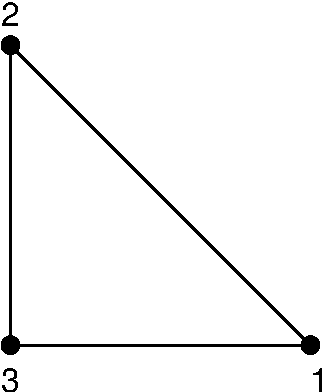
\includegraphics[width = 0.4\linewidth, viewport = 0 0 159 188]{tria3.pdf}
\caption{Linear interpolation.}
\end{minipage}
\hspace{0.5cm}
\begin{minipage}[b]{0.5\linewidth}
\centering
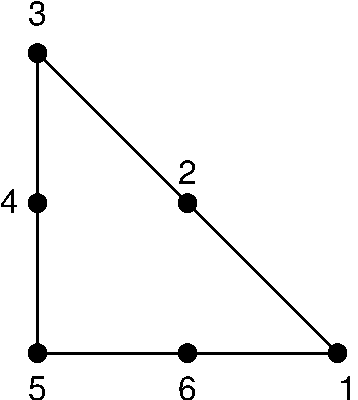
\includegraphics[width = 0.4\linewidth, viewport = 0 0 172 192]{tria6.pdf}
\caption{Quadratic interpolation.}
\end{minipage}
\end{figure}

Using this convention the shape functions for the linear case are simply given by:

\begin{eqnarray}
N_1 & = & L_1 \\
N_2 & = & L_2 \\
N_3 & = & 1-L_1-L_2
\end{eqnarray}

Under this convention the quadratic interpolation shape functions are given by:

\begin{eqnarray}
N_1 & = & L_1(2L_1-1) \\
N_2 & = & 4L_1L_2 \\
N_3 & = & L_2(2L_2-1) \\
N_4 & = & 4L2(1-L_1-L_2) \\
N_5 & = & L_3[1-2(L_1+L_2)] \\
N_6 & = & 4L_1(1-L_1-L_2)\end{eqnarray}

\pagebreak
\section{Numerical Integration}

\subsection*{Regular integrals}
For non-singular integrals the integration is done using gaussian quadrature with NG integration points per element as in:

\begin{equation}
\int_{-1}^1{F(L_1,L_2)dL_1dL_2} \approx \sum_{i=1}^{NG}{F(L_1^i,L_2^i)w_i}
\end{equation}

By default the program uses 7 points per triangular element. Tests where done with 16 and 64 points per element and the accuracy of the results was not affected, so 7 points were kept for speed.

\subsection*{Weakly singular integrals}
For weakly singular integrals the integration is done through a regularization transformation that eliminates the singularity. The element is transformed into a triangle with a singularity in node 1 and then into a degenerate square. In the degenerate square we can use Gauss-Jacobi integration to integrate getting rid of the singularity. See Figure 3 for the transformation.

\begin{equation}
\int_{-1}^1{F(L_1,L_2)(1+L_2)dL_1dL_2} \approx \sum_{i=1}^{NG}{\sum_{j=1}^{NG}{F(L_1^i,L_2^j)w_i^{\rm Gauss}w_j^{\rm Gauss-Jacobi}}}
\end{equation}

Notice that the Gauss-Jacobi integration is necessary in only one of the directions, so in the other the standard Gauss quadrature on a line is used and the product of the two provides the correct integration as indicated by the expression above.

\begin{figure}[!hbt]
\begin{center}
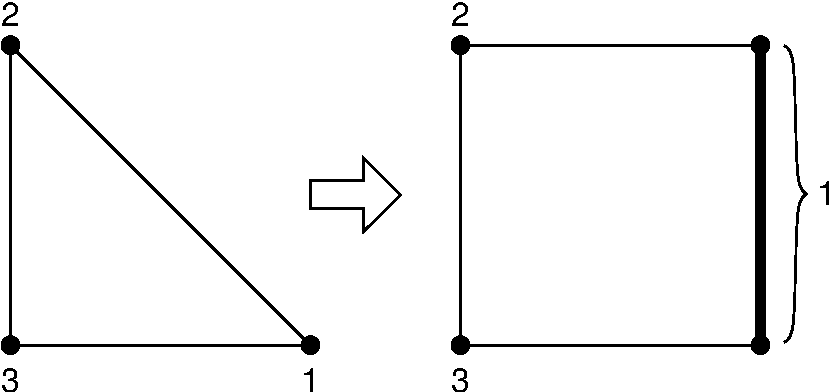
\includegraphics[width=0.6\textwidth, viewport = 0 0 402 188]{weakly_singular.pdf}
\caption{Regularization transformation for weakly singular integrals (linear case).}
\end{center}
\end{figure}

In the case of quadratic triangles when the singular point is on an edge of the triangle rather than on a vertex the triangle is divided in two and then the same regularization procedure is applied to both subtriangles as shown in Figure 4.

\begin{figure}[!hbt]
\begin{center}
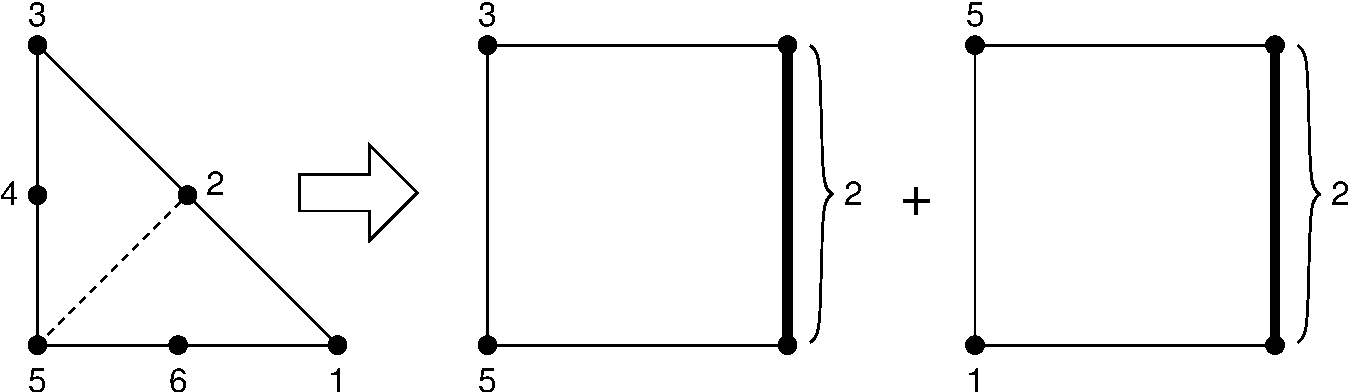
\includegraphics[width=\textwidth]{weakly_singular_t6.pdf}
\caption{Regularization transformation for weakly singular integrals (quadratic case).}
\end{center}
\end{figure}

\subsection*{Strongly singular integrals}
For strongly singular integrals we subdivide the triangle progressively in up to \verb+NSUBDIVISIONS+ --found in file \verb+constants.h+-- subsequent divisions, and integrate using standard gausian quadrature in each subtriangle except the closest to the singular point, which is neglected (it can be shown that the integrand goes to zero very close to the singularity point). The subdivision process is ilustrated in Figure 5 for a singularity at node 3 in a flat triangle.

\begin{figure}[!hbt]
\begin{center}
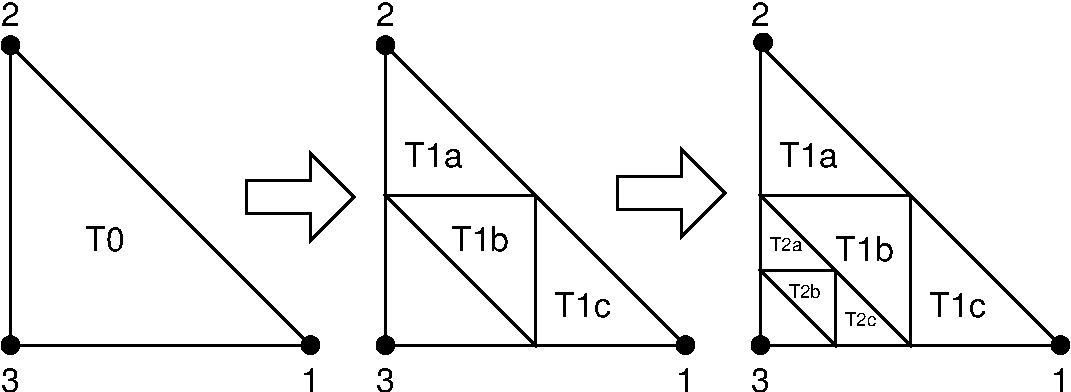
\includegraphics[width=\textwidth]{strongly_singular.pdf}
\caption{Subdivision process for strongly singular integrands with singularity at node 3 (only two consecutive subdivisions shown).}
\end{center}
\end{figure}

In the cases where the singular point is on the edge of a quadratic element rather than on a vertex the triangle is divided in two and the same subdivision process applied to the resulting subtriangles.

\subsection*{Changing the number of integration points}
The gaussian quadrature data is stored in the file \verb+gaussData.h+, and has two options, one with 7 integration points and another one with 64 integrations points. By default the code uses 7 integration points because increasing this number does not seem to improve accuracy, but this can be changed by following these steps:

\begin{enumerate}
\item Change the value of \verb+TNGAUSS+ and \verb+TSNGAUSS+ to 64 in file \verb+constants.h+
\item Comment out the 7 point \verb+TGauss+ and \verb+TSGauss+ matrices in file \verb+gaussData.h+
\item Uncomment the 64 point \verb+TGauss+ and \verb+TSGauss+ matrices in file \verb+gaussData.h+
\item Recompile the source code
\end{enumerate}

The constant values \verb+TNGAUSS+ and \verb+TSNGAUSS+ are the number of integration points in regular and strongly singular integrals, so it is also possible to use different values for them. Keep in mind that \verb+NSUBDIVISIONS+ are made in the case of strongly singular integrals, and therefore many more points are used for the integration even if \verb+TNGAUSS+ and \verb+TSNGAUSS+ are given the same value.

The numerical values of the gaussian integration are shown in the following tables.

\pagebreak
\begin{center}
\begin{tabular}{|c|c|c|c|}
\multicolumn{4}{c}{Table 1: Abscissas and weights for Gauss quadrature on a triangle}\\
\hline
NG & $x_i$ & $y_i$ & $w_i$\\
\hline\hline
7 & 0.333333333333333 & 0.333333333333333 & 0.112500000000000\\
 & 0.470142064105115 & 0.470142064105115 & 0.066197076394253\\
 & 0.059715871789770 & 0.470142064105115 & 0.066197076394253\\
 & 0.470142064105115 & 0.059715871789770 & 0.066197076394253\\
 & 0.101286507323456 & 0.101286507323456 & 0.062969590272414\\
 & 0.797426985353088 & 0.101286507323456 & 0.062969590272414\\
 & 0.101286507323456 & 0.797426985353088 & 0.062969590272414\\
\hline
\end{tabular}
\end{center}

\begin{center}
\begin{tabular}{|c|c|c|}
\multicolumn{3}{c}{Table 2: Abscissas and weights for Gauss-Jacobi quadrature on a line}\\
\hline
NG & $x_i$ & $w_i$\\
\hline\hline
8 & -0.910732089420060 & 0.013180765768995\\
 & -0.711267485915709 & 0.713716106239446\\
 & -0.426350485711139 & 0.181757278018796\\
 & -0.090373369606853 & 0.316798397969277\\
 & 0.256135670833455 & 0.424189437743720\\
 & 0.571383041208738 & 0.450023197883551\\
 & 0.817352784200412 & 0.364476094545495\\
 & 0.964440169705273 & 0.178203217446225\\
\hline
\end{tabular}
\end{center}

\begin{center}
\begin{tabular}{|c|c|c|}
\multicolumn{3}{c}{Table 3: Abscissas and weights for Gauss quadrature on a line}\\
\hline
NG & $x_i$ & $w_i$\\
\hline\hline
8 & -0.960289856497536 & 0.101228536290370\\
 & -0.796666477413627 & 0.222381034453376\\
 & -0.525532409916329 & 0.313706645877887\\
 & -0.183434642495650 & 0.362683783378362\\
 & 0.183434642495650 & 0.362683783378362\\
 & 0.525532409916329 & 0.313706645877887\\
 & 0.796666477413627 & 0.222381034453376\\
 & 0.960289856497536 & 0.101228536290370\\
\hline
\end{tabular}
\end{center}

\end{document}
